\section{The Bare Minimum}
\label{sec:bare_minimum}

\subsection{Creating a Program}
\label{sub:creating_a_program}
\begin{frame}
	\frametitle{Creating a Program}
	\begin{columns}[T]
		\begin{column}{0.5\textwidth}
			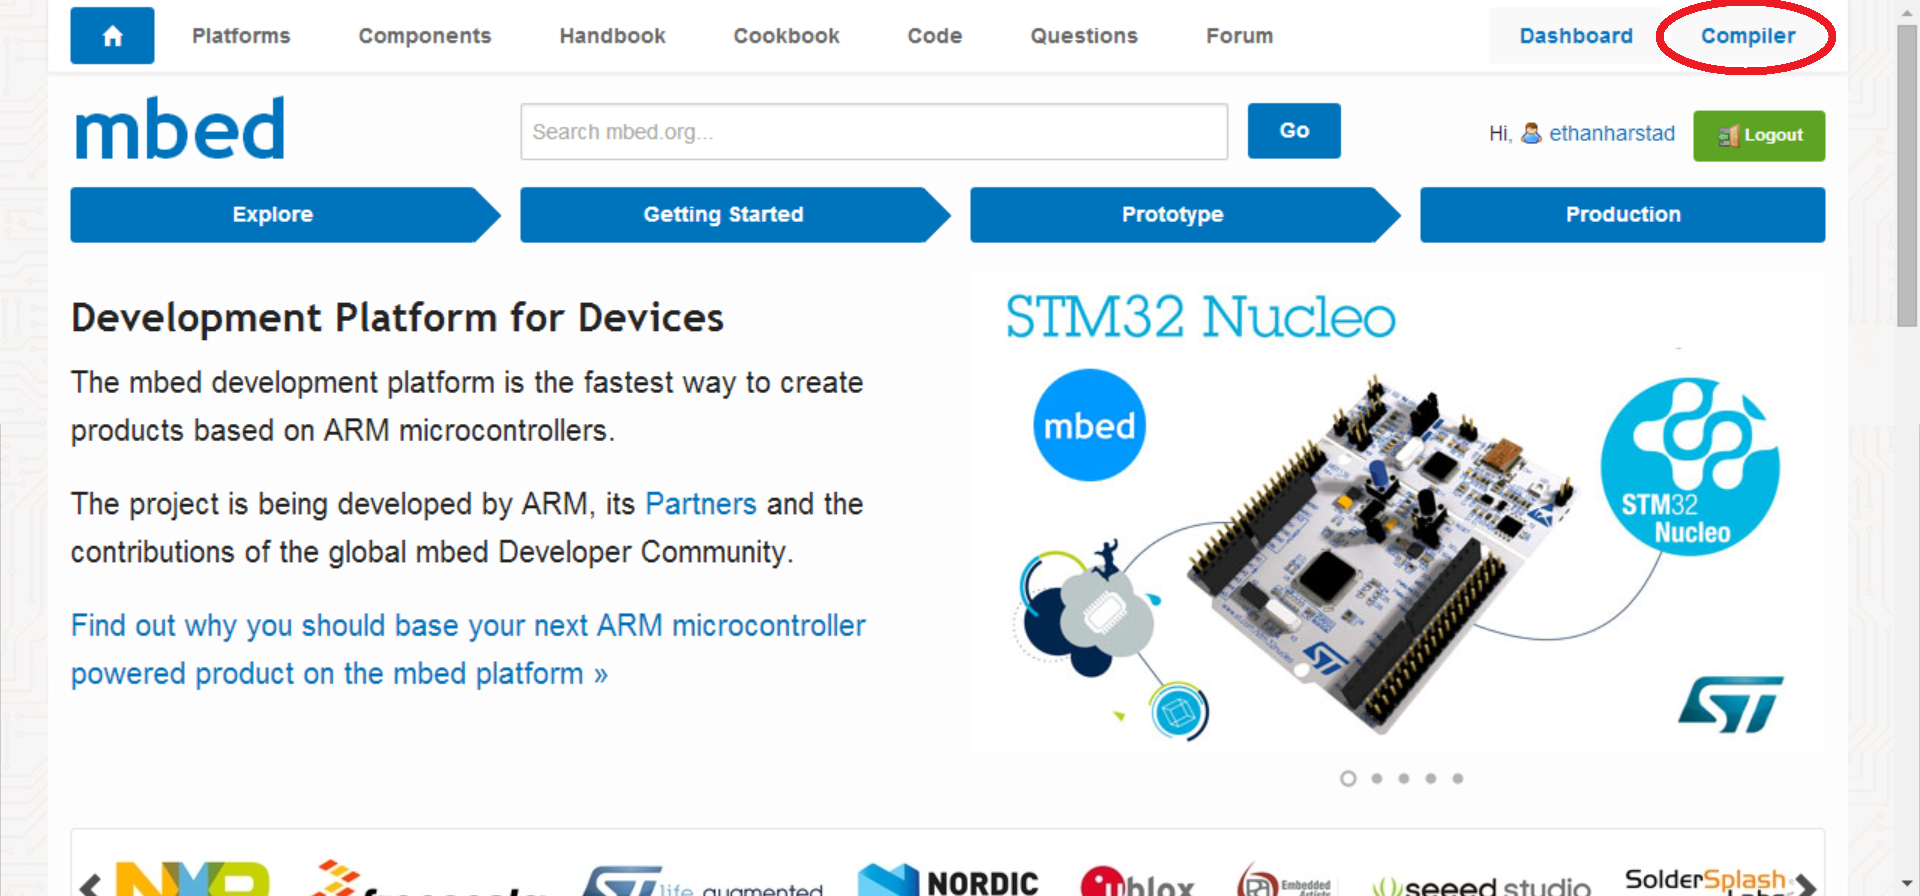
\includegraphics[width=\linewidth]{open_compiler}
			\vspace{1ex}
			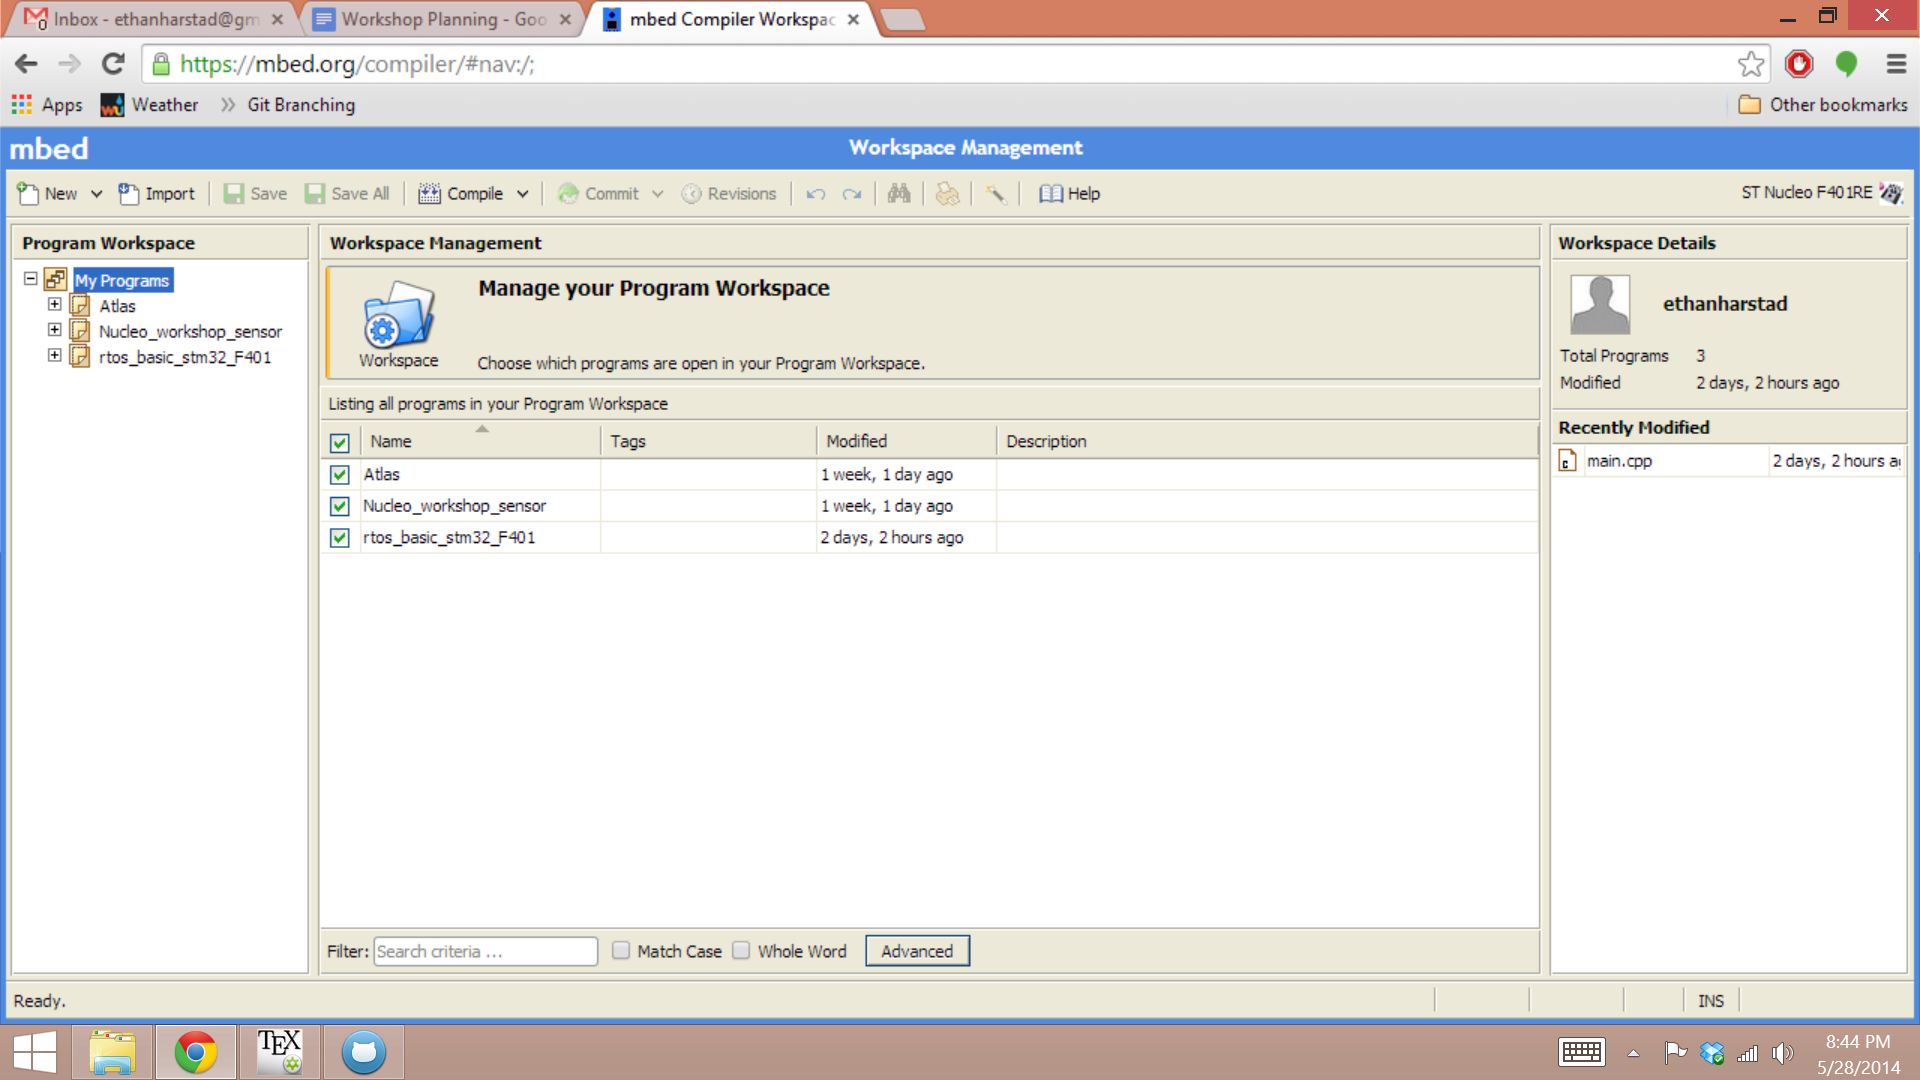
\includegraphics[width=\linewidth]{new_project}
		\end{column}
		\begin{column}{0.5\textwidth}
			\begin{enumerate}
				\item Navigate to the mbed homepage and click the "Compiler" button
				\item Click the "New" button and select "New Program"
				\item Change the Template field to "Empty Program"
				\item Give your program a name and click "OK"
			\end{enumerate}
		\end{column}
	\end{columns}
\end{frame}

\subsection{Importing a Library}
\label{sub:importing_a_library}
\begin{frame}
	\frametitle{Importing a Library}
	\begin{columns}[T]
		\begin{column}{0.5\textwidth}
			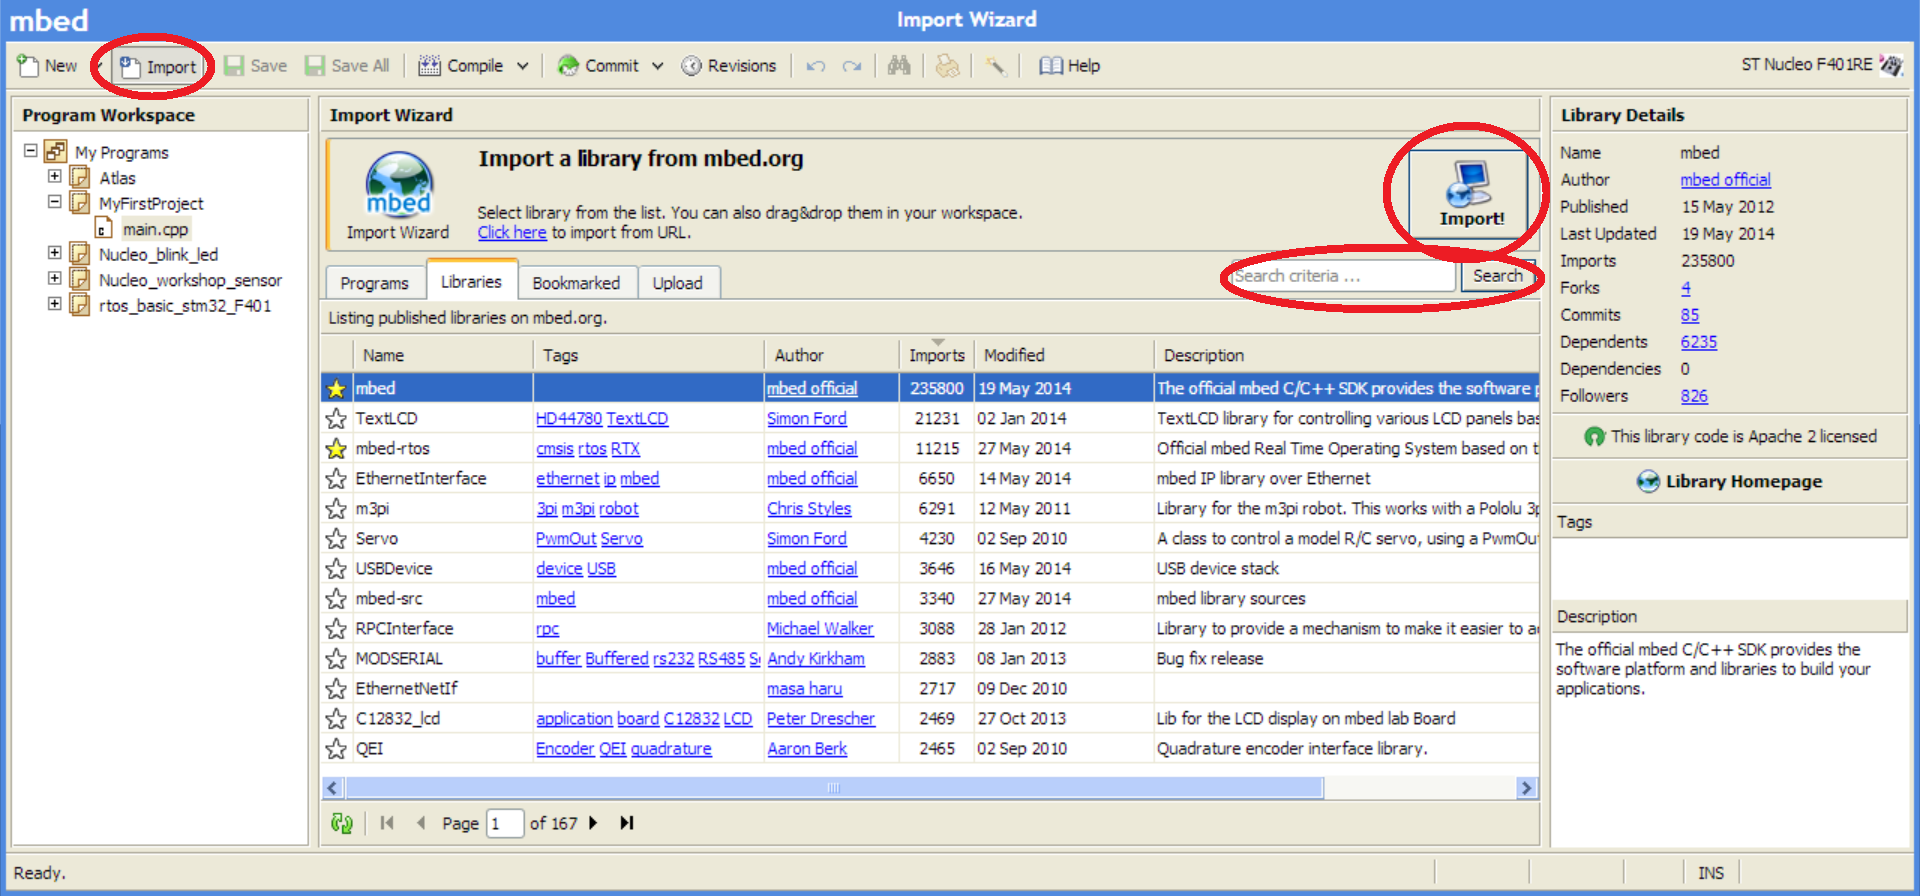
\includegraphics[width=\linewidth]{import_library}
			\vspace{1ex}
			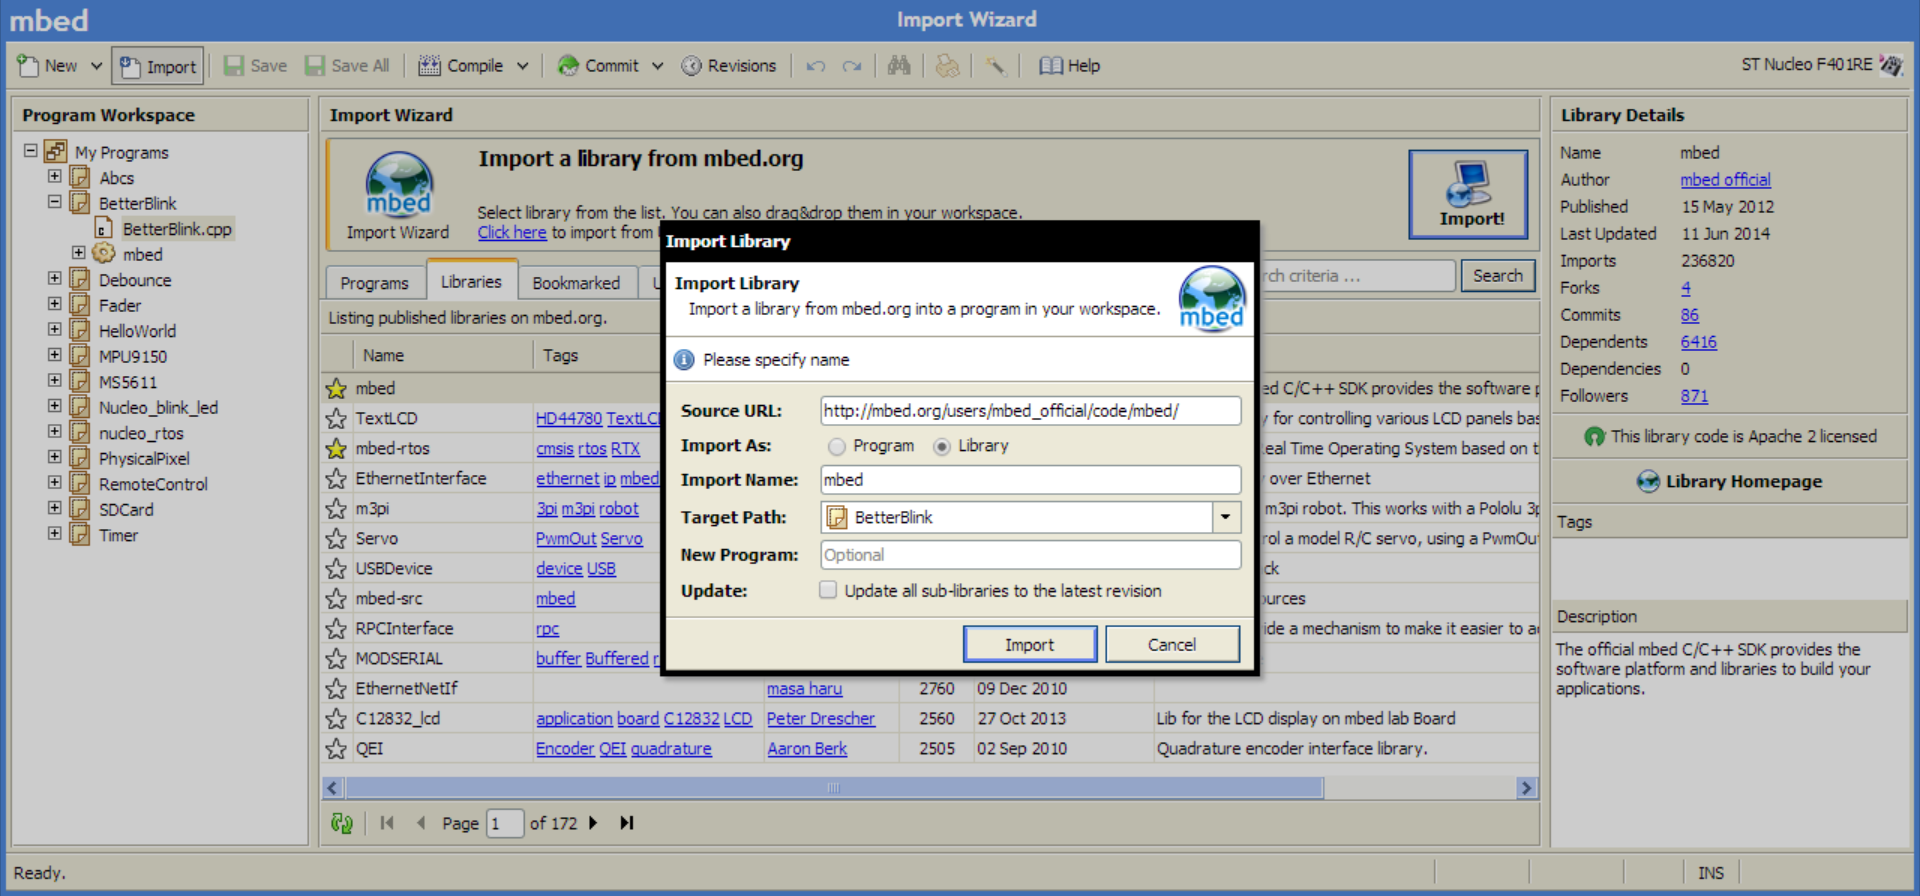
\includegraphics[width=\linewidth]{import_dialog}
		\end{column}
		\begin{column}{0.5\textwidth}
			\begin{enumerate}
				\item Click the "Import" button
				\item Search for the "mbed" library
				\item Select the library
				\item Click the "Import!" button
				\item Make sure the Target Path is your project root
				\item Click "Import" one last time
			\end{enumerate}
		\end{column}
	\end{columns}
\end{frame}

\subsection{Program Structure}
\label{sub:program_structure}
\begin{frame}
	\frametitle{Creating a New File}
	\begin{columns}[c]
		\begin{column}{0.5\textwidth}
			\begin{enumerate}
				\item Click the root directory of your project to select it
				\item Click the arrow next to "New" and select "New File"
				\item Name the file "main.cpp" and click "OK"
			\end{enumerate}
		\end{column}
		\begin{column}{0.5\textwidth}
			\begin{block}{Warning}
				Be sure to select the folder you want your file in before creating it!
			\end{block}
		\end{column}
	\end{columns}
	\begin{center}
		You can name this file anything but it must have the .cpp extension.
		It is suggested that the main file be named "main" or the same as your project name (important later on).
	\end{center}
\end{frame}

\begin{frame}
	\frametitle{Program Structure}
	\begin{columns}[c]
		\begin{column}{0.45\textwidth}
			\lstinputlisting[title=main.cpp]{code/first_program/0.cpp}
		\end{column}
		\begin{column}{0.55\textwidth}
			\begin{itemize}
				\item Line 2 includes the mbed library, \textbf{every} mbed program needs this.
				\item Line 8 is the main function, this is the entry point into your program.
					\textbf{Every} program needs a main function.
				\item Line 9 is a comment, everything after // is ignored.
				 \item Line 4-5 is a multi line comment, everything between /* */ is also ignored.
			\end{itemize}
		\end{column}
	\end{columns}
\end{frame}

\subsection{Compiling}
\label{sub:compiling}
\begin{frame}
	\frametitle{Compiling}
	\begin{columns}[c]
		\begin{column}{0.5\textwidth}
			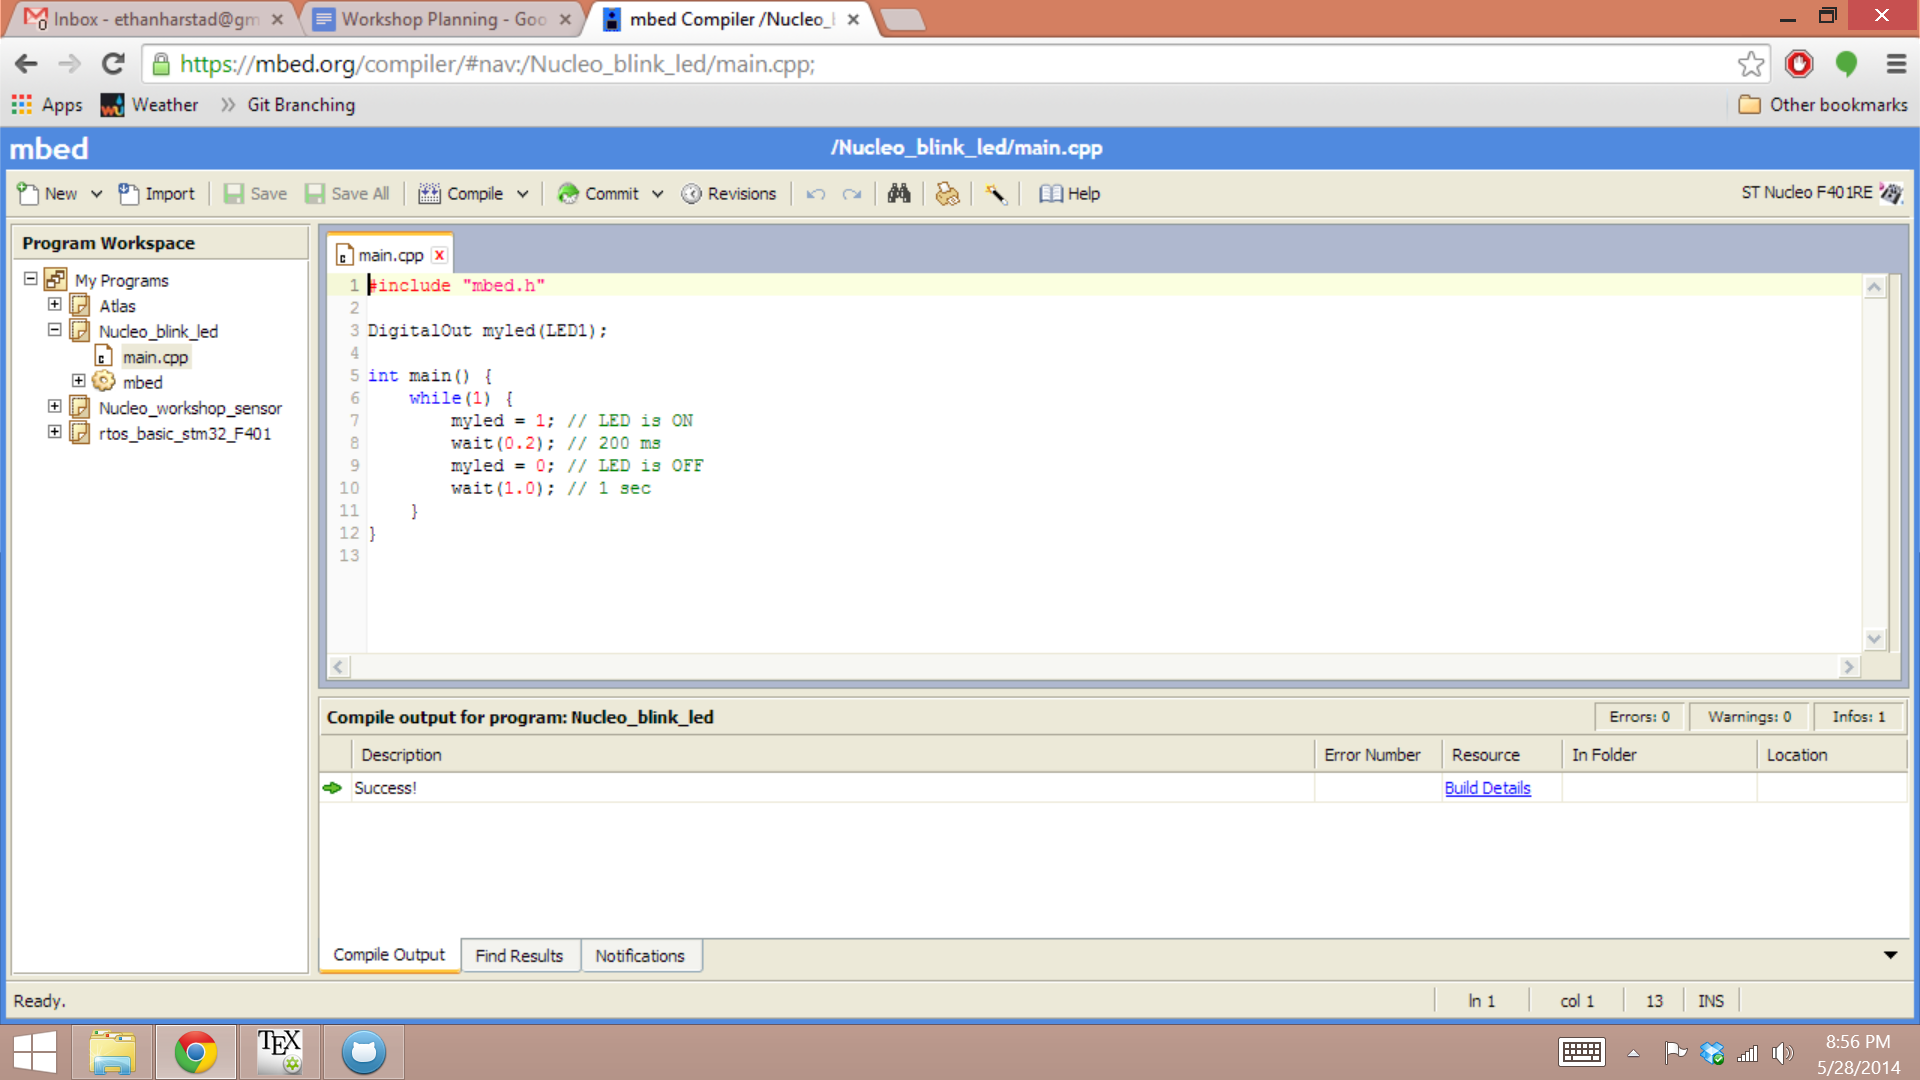
\includegraphics[width=\linewidth]{compile_program}
			\begin{block}{Tip}
				Set your browsers download location to the Nucleo to save time
			\end{block}
		\end{column}
		\begin{column}{0.5\textwidth}
			\begin{enumerate}
				\item Click "Compile" (Ctrl D) to compile your program
				\item A *.bin file will be downloaded
				\item Move the downloaded file to the Nucleo drive
				\item The Nucleo will flash red and green while programming
				\item When the lights stop, your program has started successfully!
			\end{enumerate}
		\end{column}
	\end{columns}
	\begin{center}
		You can also click "Build Only" (Ctrl B) to simply test your code
	\end{center}
\end{frame}